\section{Planificación}

La planificación del proyecto se ha realizado a partir del conjunto de historias de usuario definidas previamente, cubriendo todas las fases del desarrollo: análisis, diseño, implementación, validación y documentación.


Cada historia de usuario ha sido estimada en puntos de historia, considerando que:
\begin{itemize}
    \item 1 punto de historia equivale aproximadamente a 4 horas de trabajo.
    \item La dedicación media al proyecto ha sido de 2 horas diarias.
    \item Esto supone unas 14 horas semanales, es decir, 56 horas mensuales.
\end{itemize}



El desarrollo del proyecto se ha extendido a lo largo de \textbf{5 meses}, organizados en 4 sprints según la metodología Scrum. Aunque inicialmente se planteó una duración homogénea para los sprints, la planificación se ajustó en función de la naturaleza de las tareas. En particular, el tercer sprint presenta una mayor duración al concentrar tareas de mayor complejidad y dependencia entre sí, lo que requirió más tiempo de desarrollo y pruebas. Esta decisión permite mantener una coherencia funcional dentro del sprint y evitar la fragmentación de funcionalidades relacionadas.



La asignación de historias de usuario a cada sprint se ha realizado teniendo en cuenta su prioridad, dependencias y complejidad, permitiendo una evolución progresiva del sistema desde las funcionalidades más básicas hasta las más avanzadas, y finalizando con la documentación del proceso y el resultado. Por tanto, la planificación se estructura en los siguientes 4 sprints:

\begin{itemize}

\item \textbf{Sprint 1 (01/01/2026 – 31/01/2026)}.
En este primer sprint se han abordado principalmente tareas de análisis, investigación y definición del proyecto. Se incluyen las historias de usuario HU-02, HU-03, HU-04 y HU-05.

\textit{Esfuerzo estimado: 14 puntos.}

\item \textbf{Sprint 2 (01/02/2026 – 28/02/2026)}.
En este sprint se ha trabajado en la gestión de usuarios: registro, inicio de sesión, recuperación de credenciales, y perfiles. Se incluyen HU-08, HU-09, HU-10, HU-11, HU-12 y HU-13. En esta fase se consolida la base funcional del proyecto dado que con un sistema sólido de usuarios con acceso a la plataforma se habilita la construcción del resto de funcionalidades y su validación.

\textit{Esfuerzo estimado: 14 puntos.}

\item \textbf{Sprint 3 (01/03/2026 – 30/04/2026)}.
Este sprint se ha centrado en el núcleo del proyecto: el desarrollo de la lógica principal de correspondencia y corrección de cartas. Se incluyen once historias, de la HU-14 a la HU-24. Se trata del grueso del código, por lo que su compleción requiere una cantidad más elevada de horas de trabajo.

\textit{Esfuerzo estimado: 28 puntos.}

\item \textbf{Sprint 4 (01/05/2026 – 31/05/2026)}.
En el último sprint se han desarrollado las funcionalidades sociales de la aplicación, como la adición y eliminación de contactos y la página de Amigos; además de completar las tareas de documentación. La historias cubiertas son la HU-25, HU-26, HU-27 Y HU-28 para ese primer conjunto de tareas, y la HU-01, HU-06 y HU-07 para la parte de redacción del documento.

\textit{Esfuerzo estimado: 14 puntos.}

\end{itemize}



A continuación, se muestra un resumen de la planificación del proyecto del que se puede deducir que se emplearon un total de 280 horas (70 puntos).

\begin{table}[H]
\centering
\begin{tabular}{|c|c|c|c|}
\hline
\textbf{Sprint} & \textbf{Fechas} & \textbf{Historias de Usuario} & \textbf{Puntos} \\
\hline
Sprint 1 & Enero 2026 & HU-02 a HU-05 & 14 \\
\hline
Sprint 2 & Febrero 2026 & HU-8 a HU-13 & 14 \\
\hline
Sprint 3 & Marzo - Abril 2026 & HU-14 a HU-24 & 28 \\
\hline
Sprint 4 & Mayo 2026 & HU-25 a HU-28, HU-01, HU-06, HU-07 & 14 \\
\hline
\end{tabular}
\caption{Resumen de la planificación por sprints}
\end{table}



Para la gestión de la planificación se ha utilizado un tablero en Trello, donde las historias de usuario se han organizado en distintas columnas que reflejan su estado dentro del flujo de trabajo del proyecto.

Las columnas utilizadas han sido: \textit{Product Backlog}, que contiene todas las historias de usuario pendientes de priorización o inicio; \textit{Sprint Backlog}, que incluye las historias seleccionadas para el sprint actual; \textit{En proceso}, para aquellas que se encuentran en fase de implementación; \textit{En revisión}, donde se sitúan las funcionalidades finalizadas a la espera de validación en la Sprint Review con el tutor; y finalmente \textit{Finalizado}, donde se encuentran las funcionalidades validadas y aceptadas.

Al final de cada sprint se realiza una revisión del incremento generado junto con el tutor, en la que se valida el funcionamiento de las funcionalidades desarrolladas y se decide su aceptación o posibles mejoras.

\begin{figure}[h]
    \centering
    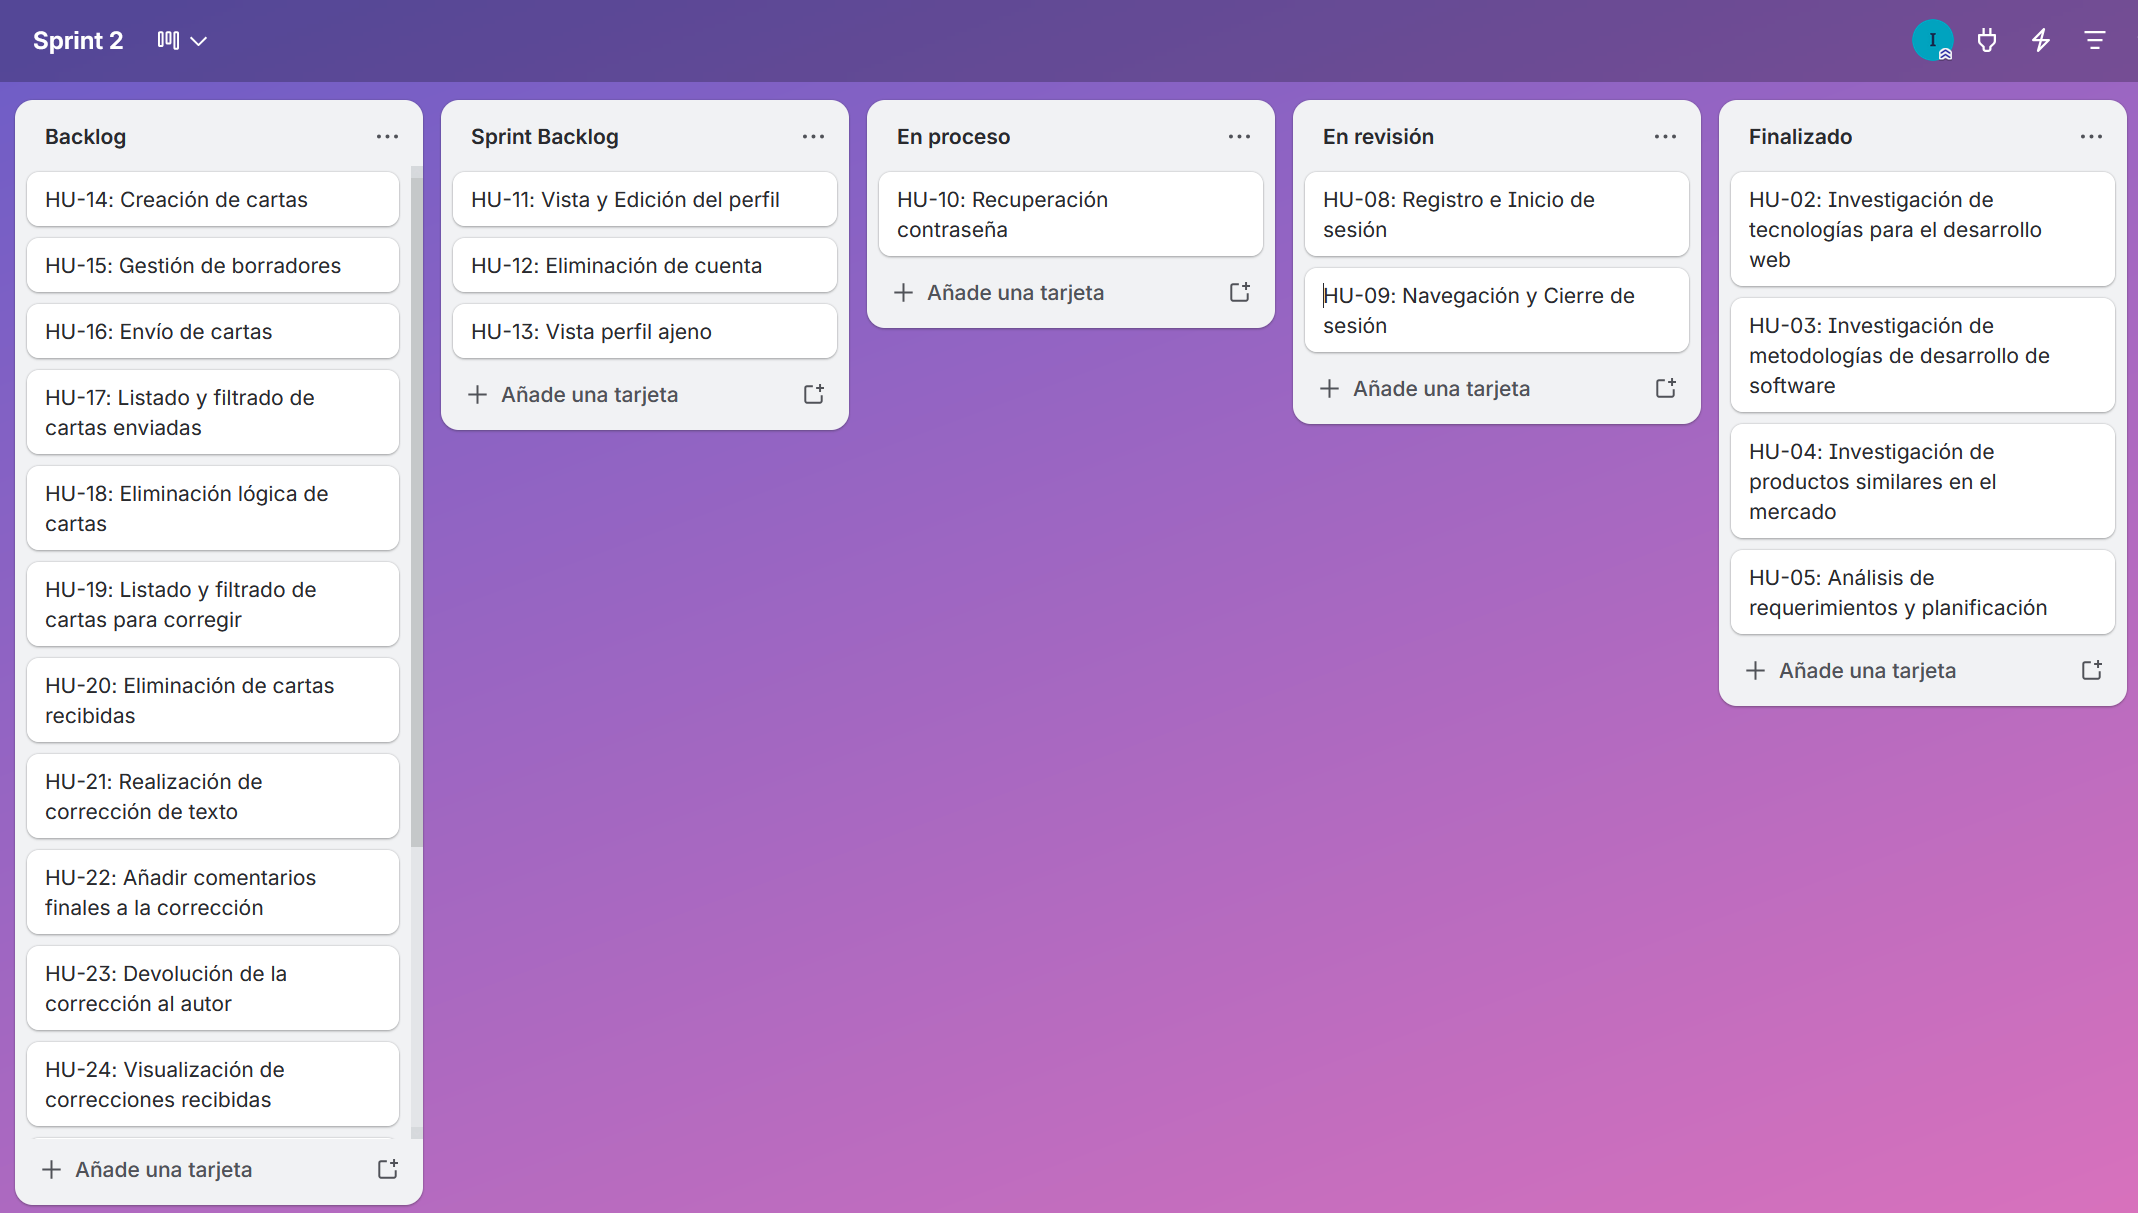
\includegraphics[width=\textwidth]{./imagenes/sprint2-trello.png}
    \caption{Ejemplo de sprint en Trello}
    \label{fig:trello}
\end{figure}


